So, we coud see interesting monotonous gap in Hye, during in arrow rotation:

\begin{figure}[h]
    \centering
    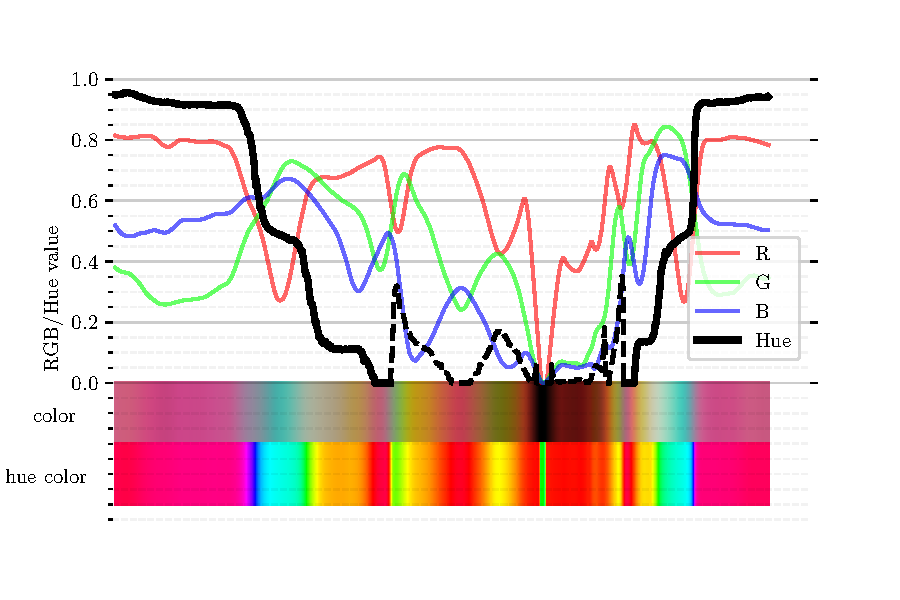
\includegraphics[width=1\textwidth]{figures/P3.pdf}
    \caption{Observed colors, RGB and Hue decomposition}
    %\label{fig:}
\end{figure}
